\documentclass{article}

\usepackage{times}
\usepackage{iclr2026_conference}
\input{math_commands.tex}

\usepackage{amsmath}
\usepackage{amssymb}
\usepackage{amsthm}
\usepackage{booktabs}
\usepackage{graphicx}
\usepackage{tabularx}
\usepackage{url}
\usepackage[hidelinks]{hyperref}

\title{Certified TailGuard for Vision-Language-Action Selection}

\author{Anonymous authors}

\newtheorem{theorem}{Theorem}
\newtheorem{proposition}{Proposition}
\newcommand{\method}{Certified TailGuard}
\newcommand{\sem}{S_{\mathrm{sem}}}
\newcommand{\phys}{S_{\mathrm{phys}}}
\newcommand{\calib}{S_{\mathrm{cal}}}
\newcommand{\util}{R}

\begin{document}

\maketitle

\begin{abstract}
Vision-language-action (VLA) policies increasingly combine language-conditioned action generation with inference-time selection among multiple candidates. This paper studies a controlled failure mode of that selection step. In a finite candidate pool, top-score selection is governed by the physical utility of the selected score tail, not by average semantic plausibility. We give an exact tie-aware finite-pool law and use it to define semantic affordance over-selection: selected language/vision plausibility rises with $N$ while selected physical utility saturates or collapses. We then introduce \method{}, an abstaining inference-time controller that hard-filters candidates with modeled physical certificates, calibrates selected-tail utility from pilot labels, applies lower confidence bounds, compares against $N=1$ and random-selection baselines, and either allows high $N$, stops early, requests labels, or blocks high $N$. Controlled VLA-style, rendered-simulator, robustness, phase-diagram, and ablation artifacts support the selected-tail claim and show controlled repair only when the modeled certificates cover the relevant failure modes. External RoboCasa/LIBERO artifacts are reported as integration status only; they contain no reward/success metrics, no external method outcome, and no hardware validation.
\end{abstract}

\section{Introduction}

VLA systems map an instruction and visual observation to robot actions or trajectories. Modern robot foundation models make this interface compelling because semantic knowledge can help a policy choose the right object, receptacle, or tool \citep{ahn2022saycan,brohan2022rt1,brohan2023rt2,kim2024openvla}. Deployment, however, often adds an inference-time selection layer: sample several candidate actions, score them, and execute the top-ranked candidate. This layer can help when the score's upper tail is physically meaningful. It can hurt when the score is mostly semantic and the top semantic tail contains unreachable, collision-prone, wrong-object, or wrong-receptacle actions.

The core claim is narrow. For a fixed VLA-style generator and scorer, increasing $N$ stresses the selected score tail. If that tail is misaligned with physical utility, selected semantic plausibility can improve while real utility drops. Average score-utility correlation, imitation loss, or language plausibility is not enough to certify high-$N$ action selection. The selected tail itself must be audited.

We make three contributions. First, we state and validate an exact finite, tie-aware score-tail law for selected utility under sampling without replacement. Second, we build controlled VLA-style diagnostics that separate instruction/vision/action semantic scores from physical utility and violations. Third, we introduce \method{}, a conservative inference-time controller that uses modeled physical certificates, pilot-label calibration, empirical lower bounds, and abstention to prevent high-$N$ overclaims. The paper's evidence is intentionally controlled. Optional SmoLVLA, RoboCasa, and LIBERO artifacts record plumbing and integration boundaries, but the paper reports no benchmark outcomes and no hardware outcomes.

\section{Finite Selected-Tail Law}

Let a fixed candidate pool contain $m$ actions $a_i$ generated from observation $o$ and instruction $\ell$. Each candidate has a selection score $s_i$ and physical utility $r_i \in [0,1]$. A top-score selector samples $N$ distinct candidates uniformly without replacement and selects a uniformly random member among sampled candidates with maximal score.

\begin{theorem}[Tie-aware finite score-tail law]
For candidate $i$, let $e_i = |\{j:s_j=s_i\}|$ and $\ell_i=|\{j:s_j<s_i\}|$. Its exact selection probability is
\[
p_i(N)=\frac{1}{e_i}\sum_{k=\max(1,N-\ell_i)}^{\min(e_i,N)}
\frac{\binom{e_i}{k}\binom{\ell_i}{N-k}}{\binom{m}{N}},
\]
with impossible binomial terms omitted. Therefore the expected selected utility is
\[
\mathbb{E}[\util(a_{\mathrm{sel}})] = \sum_{i=1}^{m} p_i(N) r_i .
\]
\end{theorem}

The law makes the selected-tail principle explicit: as $N$ grows, probability mass moves to high-score candidates. High-$N$ utility is therefore governed by $\mathbb{E}[\util\mid s \text{ lies in the selected upper tail}]$, not by global score quality. If a semantic scorer ranks plausible but physically bad actions at the top, more samples can make the selected action look better to the semantic scorer and worse to the robot.

In our VLA-style setup, $s_i$ may be a semantic affordance score $\sem(o,\ell,a_i)$, a physical score $\phys(o,a_i)$, or a calibrated score $\calib(o,\ell,a_i)$. The real utility $\util(a_i)$ is always evaluated separately. Diagnostics include selected semantic score, selected real utility, exact-law prediction error, high-$N$ regret, oracle gap, violation rate, wrong-object and wrong-target rates, reachability, collisions, stability, fragile/heavy failures, and tail rank correlation.

\section{\method{}}

\method{} is an inference-time gate for finite candidate pools. It does not train a new VLA and does not assume semantic score is a safety signal. Given semantic scores, optional verifier scores, pilot real-utility labels, modeled physics flags, and a candidate $N$ grid, the controller returns one of four public decisions: \texttt{allow\_high\_n}, \texttt{stop\_early}, \texttt{collect\_pilot\_labels}, or \texttt{block\_high\_n}.

The first layer is a hard certificate. A candidate must pass modeled predicates for reach envelope, swept collision, receptacle compatibility, stability margin, fragile/heavy handling, tool-object match, blocked-path constraints, and modeled hidden obstacles. These predicates are deliberately local to the controlled simulator. They are not real-world safety certificates.

The second layer fits a bounded calibrator from pilot labels. Features include semantic score, physical/verifier score, interactions, and score gaps. The calibrator predicts real utility for each candidate, while an empirical-Bernstein-style radius \citep{maurer2009empirical} converts selected-tail predictions into lower confidence bounds. The exact finite law is then applied to certified candidates to predict utility across the $N$ grid.

The final layer compares the lower-bound curve against two baselines: certified $N=1$ and random certified selection. High $N$ is allowed only if the lower bound beats both baselines by a margin. If high $N$ is not worth the margin, the controller stops early. If selected-tail labels are too scarce or the lower bound is too wide, it requests pilot labels. If the certified set is too small or the high-$N$ lower bound is below baselines, it blocks high-$N$ and falls back to low-$N$ certified selection when possible.

\begin{figure}[t]
\begin{center}
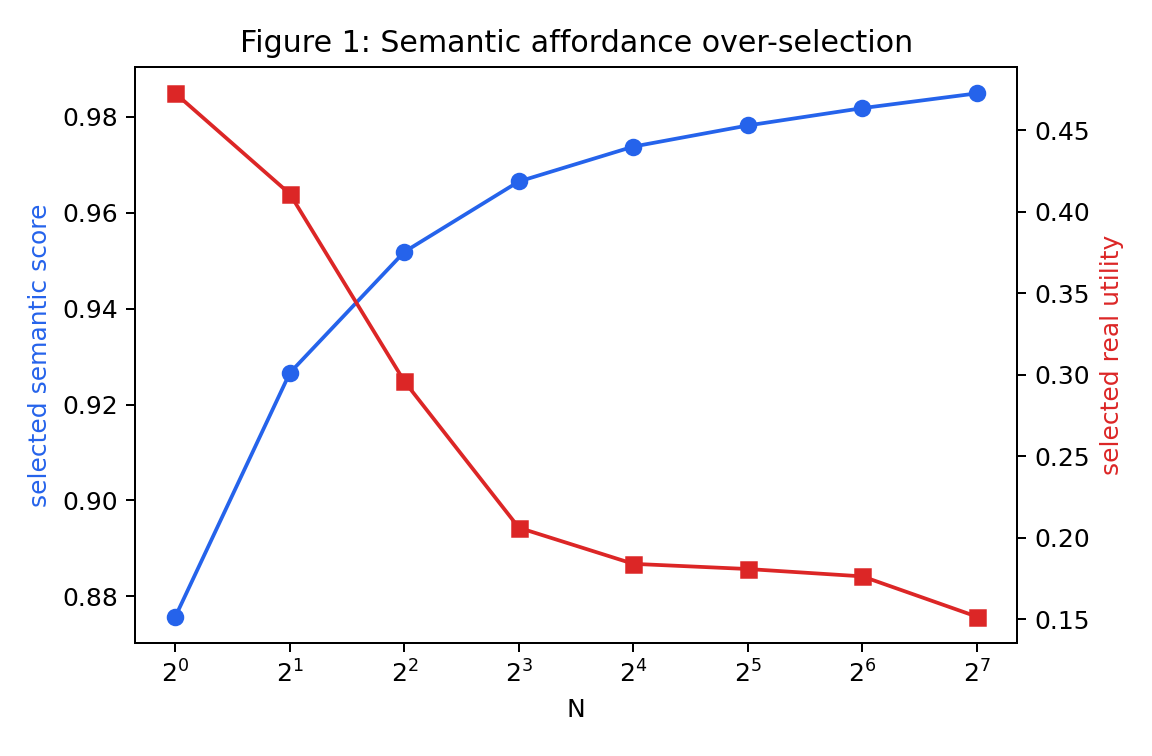
\includegraphics[width=0.48\linewidth]{../../results/figures/figure1_semantic_overselection.png}
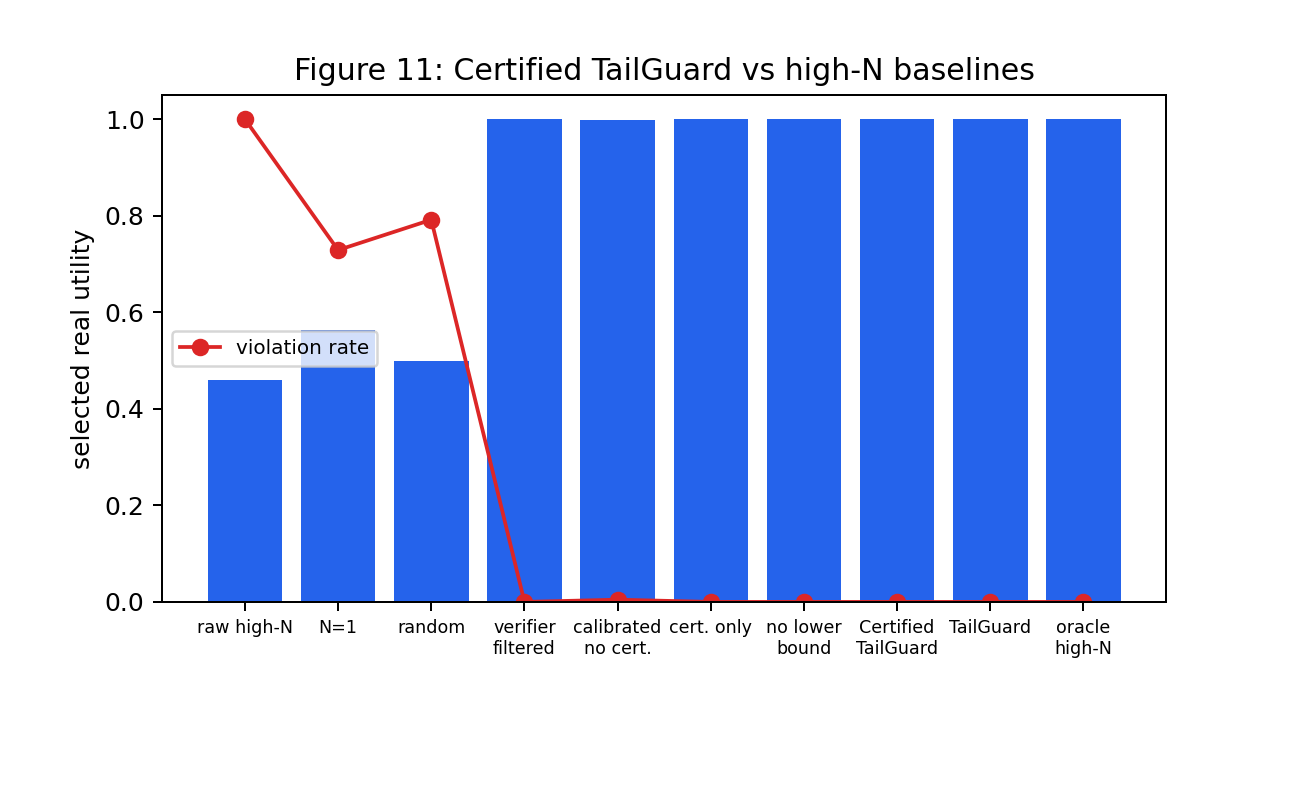
\includegraphics[width=0.48\linewidth]{../../results/figures/figure11_tailguard_adaptive_n.png}
\end{center}
\caption{Left: controlled selected-tail failure. The semantic score improves with $N$ while physical utility falls. Right: \method{} chooses or blocks $N$ using certified selected-tail lower bounds rather than raw semantic maxima.}
\label{fig:tail}
\end{figure}

\section{Evidence}

\subsection{Controlled selected-tail failure}

The controlled scenes include instructions, object colors and categories, receptacles, obstacles, reachability envelopes, collisions, fragile/heavy constraints, tool constraints, wrong-object distractors, and wrong-target receptacles. The learned VLA-style scorers consume instruction features, visual/object observation features, and action-candidate features, but are trained on semantic labels rather than real physical utility.

Table~\ref{tab:failure} shows the central failure. For the learned raw semantic scorer, selected semantic score rises from $0.876$ at $N=1$ to $0.985$ at $N=128$, while selected physical utility falls from $0.473$ to $0.152$ and violations rise to $0.958$. A PyTorch learned semantic scorer reduces but does not remove the problem: at $N=128$, utility is $0.329$ with violation $0.958$. Rendered visual scenes with simulator-style physical utility reproduce the same direction: raw high-$N$ selection reaches semantic score $0.985$, utility $0.460$, and violation $1.000$.

\begin{table}[t]
\caption{Selected-tail failure. Values are artifact rows from \texttt{results/learned\_summary.csv} and \texttt{results/rendered\_summary.csv}.}
\label{tab:failure}
\begin{center}
\small
\begin{tabular}{llrrrrr}
\toprule
Setting & Method & $N$ & Sem. & Utility & Viol. & Regret \\
\midrule
Learned & raw semantic & 1 & 0.876 & 0.473 & 0.725 & 0.000 \\
Learned & raw semantic & 128 & 0.985 & 0.152 & 0.958 & 0.848 \\
Learned & PyTorch semantic & 128 & 0.971 & 0.329 & 0.958 & 0.671 \\
Rendered & raw semantic & 1 & 0.876 & 0.564 & 0.729 & 0.000 \\
Rendered & raw semantic & 128 & 0.985 & 0.460 & 1.000 & 0.540 \\
\bottomrule
\end{tabular}
\end{center}
\end{table}

\subsection{Repair is selected-tail repair}

Table~\ref{tab:repair} compares high-$N$ repair methods at $N=128$. Physical scoring, pilot-label calibration, and grounded combined scoring repair the controlled selected tail. The important qualification is that these methods work when the modeled physical or pilot-label evidence actually changes the selected tail. Robustness artifacts show that mild noisy verification can improve utility while remaining unsafe, harsh noisy verification can fail, and calibration can become label-budget or noise limited. This is why the controller exposes \texttt{collect\_pilot\_labels} and \texttt{block\_high\_n} decisions instead of always returning a high-$N$ action.

\begin{table}[t]
\caption{Controlled high-$N$ repair at $N=128$ from \texttt{results/repair\_summary.csv}.}
\label{tab:repair}
\begin{center}
\small
\begin{tabular}{lrr}
\toprule
Method & Selected utility & Violation rate \\
\midrule
Raw semantic & 0.152 & 0.958 \\
Semantic plus physical & 0.965 & 0.042 \\
Calibrated & 0.999 & 0.058 \\
Grounded combined & 1.000 & 0.000 \\
PyTorch semantic & 0.329 & 0.958 \\
PyTorch calibrated & 0.999 & 0.060 \\
\bottomrule
\end{tabular}
\end{center}
\end{table}

\subsection{Certified TailGuard stress}

In the TailGuard stress setting, raw fixed high-$N$ selection has utility $0.460$ and violation $1.000$. The \method{} row reaches controlled utility $1.000$ with violation $0.000$, but its dominant decision is \texttt{block\_high\_n}: it falls back rather than declaring raw high-$N$ safe. Component ablations remove the physical certificate, verifier score, pilot labels, empirical lower bound, adaptive $N$, or abstention/fallback. Each named removal fails the controlled acceptance target in at least one constructed regime, while the full controller passes the corresponding row. Phase diagrams sweep semantic/physical misalignment, distractor salience, obstacle density, hidden constraints, verifier errors, label noise, and label budget.

\begin{figure}[t]
\begin{center}
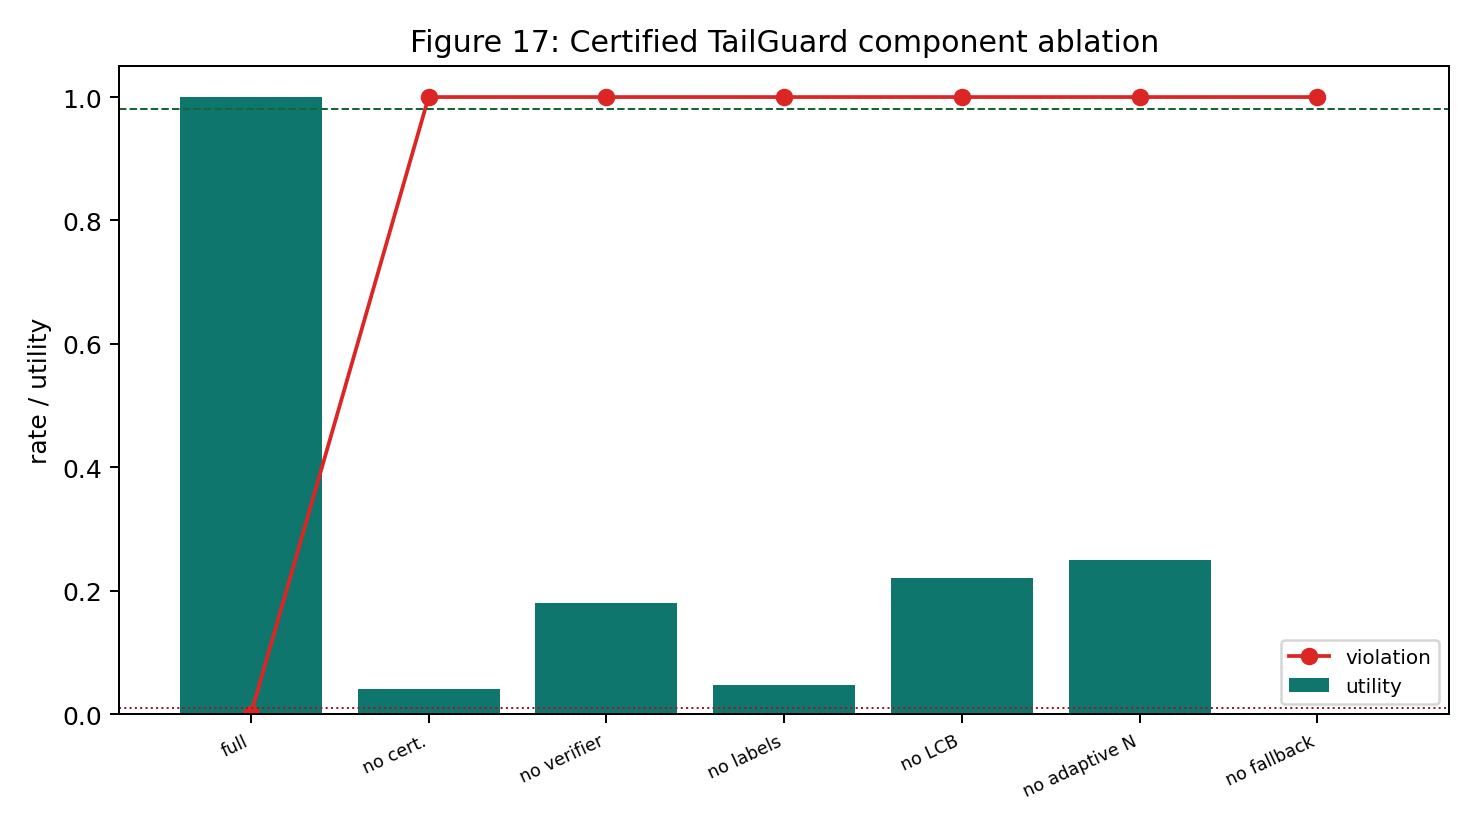
\includegraphics[width=0.48\linewidth]{../../results/figures/figure17_component_ablation.png}
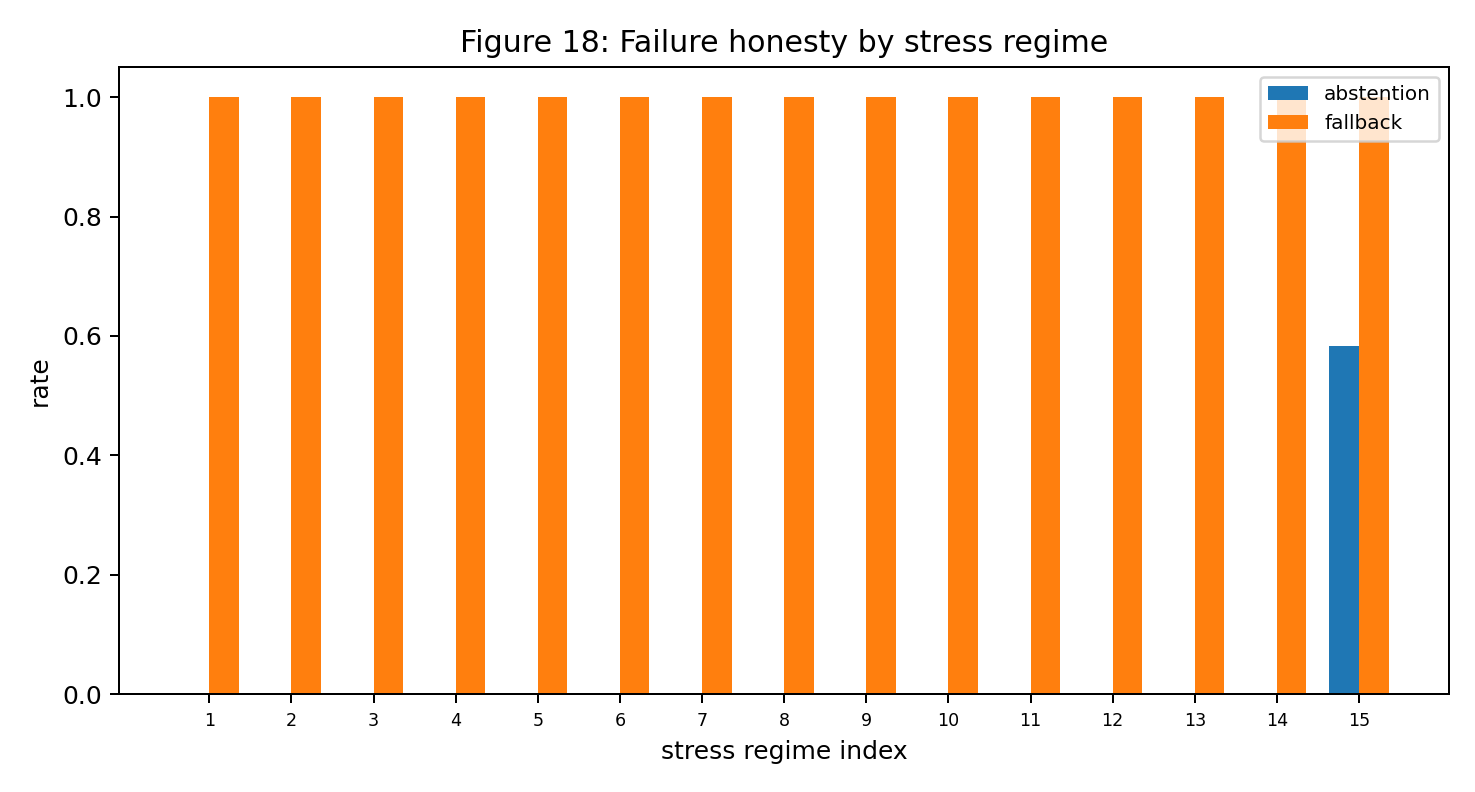
\includegraphics[width=0.48\linewidth]{../../results/figures/figure18_failure_honesty.png}
\end{center}
\caption{Ablations and failure honesty. The controller is evaluated by whether it keeps controlled utility high and violations low, and by whether it falls back or abstains in unsupported regimes. The right panel indexes rows from \texttt{failure\_honesty\_summary.csv}.}
\label{fig:ablation}
\end{figure}

\subsection{External boundary}

The external benchmark runner is artifact-gated. The current RoboCasa status records an attempted PickPlaceCounterToCabinet reset/step probe that timed out before reward or success metrics. The LIBERO row records import/status information only and no guarded reset/step wrapper. The SmoLVLA artifact records synthetic CPU action emission, not physical success. These artifacts support integration-status statements only. They do not support external simulator performance, TailGuard method success on external benchmarks, or hardware-outcome statements.

\section{Limits, Reproducibility, and Ethics}

The strongest limitation is evidence scope. The experiments are controlled, including rendered scenes and simulator-style geometry. The learned models are VLA-style semantic scorers, not deployed robot foundation models. The certificates cover only modeled predicates; unmodeled perception errors, dynamics, contact, calibration, and hardware failures are outside the guarantee. Pilot labels are assumed to measure real utility for the controlled scenes, and confidence bounds depend on selected-tail coverage. A controller that abstains may be operationally inconvenient, but in this setting abstention is the correct output when high-$N$ evidence is weak.

Reproduction uses \texttt{pytest}, the claim-audit script, and guarded external status checks. The paper-critical tables are generated from the claims, TailGuard, ablation, and related CSV/JSON artifacts under \texttt{results/}. Code can be provided as anonymous supplementary material. This work should not be used as a hardware safety guarantee; it is a diagnostic and controller study for controlled VLA-style selected-tail failures. A separate LLM usage disclosure appears in Appendix~\ref{app:llm}.

\label{page:maintextend}
\bibliographystyle{iclr2026_conference}
\bibliography{references}

\appendix

\section{Proof Details}

\begin{proof}[Proof of Theorem 1]
For a fixed score level $s$, a sampled subset selects a candidate from that level exactly when it includes no candidate with score larger than $s$ and at least one candidate with score equal to $s$. If $k$ equal-score candidates and $N-k$ lower-score candidates are sampled, there are $\binom{e_i}{k}\binom{\ell_i}{N-k}$ such subsets. The denominator is the total number $\binom{m}{N}$ of sampled subsets. Conditional on this event, tie-breaking is uniform over the $e_i$ candidates in the score group by symmetry, giving the stated $1/e_i$ factor. Expected selected utility follows by linearity.
\end{proof}

\begin{proposition}[Semantic-score no-free-lunch]
No controller that observes only semantic scores can guarantee high-$N$ physical utility when upper-tail physical utility is unconstrained.
\end{proposition}

\begin{proof}
Construct two finite pools with identical semantic scores and identical nonsemantic metadata visible to the controller. In one pool, assign utility one to the top semantic tail and zero elsewhere. In the other, assign utility zero to the same top semantic tail and one elsewhere. A semantic-only controller must make the same high-$N$ decision on both pools, so it fails on at least one. Physical certificates, verifier evidence, pilot labels, or abstention are necessary to distinguish the pools.
\end{proof}

\section{Claim-Evidence Table}

\begin{center}
\small
\begin{tabularx}{\linewidth}{p{0.30\linewidth}p{0.18\linewidth}X}
\toprule
Statement & Status & Artifact boundary \\
\midrule
Exact finite score-tail law & Supported & \texttt{theory.py}; \texttt{test\_theory.py}. \\
Semantic affordance over-selection & Supported & Controlled, learned, and rendered summary CSVs show semantic score rising while utility drops or violations rise. \\
\method{} controlled repair & Supported & \texttt{tailguard\_summary.csv}: controlled utility $1.000$, violation $0.000$ in the supported TailGuard row. \\
Component necessity & Supported & \texttt{component\_ablation\_summary.csv}: each named removal fails at least one stress regime. \\
Failure honesty & Supported & \texttt{failure\_honesty\_summary.csv}: fallback or abstention occurs in unsupported regimes. \\
External simulator outcomes & Not reported & \texttt{external\_benchmark\_status.json} has no reset/step reward success artifact. \\
Hardware validation & Not reported & No hardware or seed-level robot outcome artifact exists. \\
\bottomrule
\end{tabularx}
\end{center}

\section{External Benchmark Boundary}

The external runner records claim levels separately: integration, benchmark stepping, reward trace, exposed success metric, physical success, and TailGuard method success. Current artifacts set integration to true but benchmark stepping, success metric exposure, physical success, and TailGuard method success to false. Upgrading the claim would require reset-ok, step-ok, nonempty reward traces, exposed success metrics, an action-schema mapping, TailGuard-connected policy rows, and seed-level outcome files.

\section{LLM Usage Disclosure}
\label{app:llm}

Large language models were used substantially during manuscript preparation and repository documentation. Assistance included organizing the claim-evidence audit, drafting and editing prose, and helping implement guarded artifact checks and build automation. The authors remain responsible for all claims, experiments, code, references, and text, and verified the submission against the recorded artifacts before release.

\end{document}
